\documentclass[12pt,twoside=off,
bibtotoc,liststotoc,appendixprefix,paper=a4,headings=small]{scrbook} % 'twoside=on' für Druckversion oder 'twoside=off' für Onlineversion

%
% Packages
% -----------------------------------
\usepackage[
  paper=a4paper,
  left=12.5mm,
  right=25mm,
  top=25mm,
  bottom=50mm,
  bindingoffset=10mm]{geometry}		% Seitenränder und Bindungskorrektur einstellen
  
\usepackage{natbib}		

\setcitestyle{round,aysep={}} 		% Indizierg. in runden Klammern, zw. Autor u. Jahr
\usepackage[utf8]{inputenc}         % Umlaute im Text
\usepackage[T1]{fontenc}
\usepackage{lmodern}				% Schriftfamilie
\usepackage{microtype}				% für die Mikrotypografie (besseres Schriftbild)
\setkomafont{disposition}{\bfseries}

\usepackage{graphicx} 				% Grafiken einfügen (pdf,png - aber jpg vermeiden)
\graphicspath{{./Bilder/}}          % Pfad zu den Bildern

\usepackage{url}					% URL's formatieren (z.B. in Literatur) 
\usepackage[colorlinks,linkcolor=black,citecolor=black,urlcolor=black]{hyperref} 				% für Hyperlinks in PDF-Dokumenten   
  
\usepackage{tabularx} 				% bessere Gestaltung von Tabellen
\usepackage{longtable} 		
\usepackage{multicol}				
\usepackage{multirow}
\usepackage{booktabs}
\usepackage{tabularx}
		
\usepackage[active]{srcltx}

\usepackage{listings}				% Algorithmen

\usepackage{mdwlist}				% Listen

\usepackage{setspace} 				% Zeileneinstellung
\newtheorem{mydef}{Merksatz}  		% Falls Beispiele, Merksätze m. fortl. Nr. gebr. werden
\newtheorem{bsp}{Beispiel}

\usepackage{todonotes}				% zum Erstellen von ToDos im Editor

\usepackage{lscape}					% zum Rotieren von Seiten

\usepackage{amsmath}				% zum Schreiben von mathematischen Formeln

\usepackage{calc}

\usepackage{footnote}				% Fußnoten
\usepackage{tablefootnote}			% Fußnoten in Tabellen

%\clubpenalty = 10000
%\widowpenalty = 10000 \displaywidowpenalty = 10000

\hyphenation{voll-st\"andigen}		% Worttrennungen global definieren

\setcounter{tocdepth}{1}			% Ebenen, die im Inhaltsverzeichnis angezeigt werden

% Document
% -----------------------------------
\begin{document}

\frontmatter 
    % Titelseite soll keine Kopf oder Fußzeile haben
\thispagestyle{empty}

% Alle Elemente sollen zentriert sein
\begin{center}

\vspace*{-10mm}

{\Large \textbf{Detecting Gender Bias in}}\\ 
\vspace*{2mm}
{\Large \textbf{English-German Translations}}\\ 
\vspace*{2mm}
{\Large \textbf{using Natural Language Processing}}\\

\vspace*{\fill} 

{\LARGE {Bachelor's Thesis}}\\ 

\vspace*{\fill} 

for the attainment of the academic degree Bachelor of Science (B.Sc.)\\ \vspace*{1.5mm} 
in the study program\\\vspace*{1.5mm}
\textbf{Information Systems Management}\\\vspace*{1.5mm}
at the\\\vspace*{1.5mm}
Berlin School of Economics and Law\\

\vspace*{\fill} 

% Name des/der Autors/Autoren
{\Large Submitted by Khanh Linh Pham}\\[15mm]

\vspace*{\fill} 

% Gutachter, Kontaktdaten und Abgabetermin
\begin{flushleft}
\begin{tabbing}
Main Supervisor:\hspace{1.6cm} \= Prof. Dr. Diana Hristova \\
Secondary Supervisor:\> Prof. Dr. Markus Schaal \\[4mm]
Semester:\> Summer Semester 2025\\
Matriculation no.:\> 77211916753\\
Email:\> klpham04@gmail.com\\[8mm]
\textbf{Date of Submission:} \> \textbf{xx.xx.2025}\\
\end{tabbing}
\end{flushleft}

\end{center}

\clearpage{\pagestyle{empty}\cleardoublepage} 			% Titelblatt
    \clearpage{\pagestyle{empty}\cleardoublepage}
    \thispagestyle{empty}


\vspace*{1cm}

\begin{center}
    \textbf{Abstract}
\end{center}

\vspace*{1cm}

\noindent 
Gender bias in English–German Machine Translation often appears in forms such as generic masculine defaulting and occupation stereotyping. These biases can perpetuate unequal representations and feed back into future translation models, reinforcing biased outputs in society. This thesis examines how accurately multilingual BERT (mBERT) can detect such bias. The model was fine-tuned on limited datasets with varying annotation quality, which caused its main limitations. The classifier occasionally (1) misclassifies German gender-fair language forms as biased, (2) fails to detect bias in political and government terms, (3) fails to recognize semantically gendered words as unbiased, (4) is sensitive to punctuation and capitalization, and (5) struggles with sentences that contain both neutral and gendered subjects. Despite these gaps, the model achieved an F1 score of 0.966 and proves effective for core bias cases. It reached 84.4\% accuracy on a small handcrafted evaluation dataset with practical sentences like job postings and edge cases. As an intermediary step, the work offers a trained model, sufficiently effective for practical bias detection, and an application that make biased translations visible while indicating areas for further investigation and improvement.
    \newpage
    
    \clearpage{\pagestyle{empty}\cleardoublepage}
    \thispagestyle{empty}


\vspace*{1cm}

\begin{center}
    \textbf{Sperrvermerk}
\end{center}

\vspace*{1cm}

\noindent 

Die vorgelegte Masterarbeit basiert auf internen, vertraulichen Daten und Informationen des Unternehmens ...... In diese Arbeit dürfen Dritte, mit Ausnahme der Gutachter und befugten Mitgliedern des Prüfungsausschusses ohne ausdrückliche Zustimmung des Unternehmens und des Verfassers keine Einsicht nehmen. Von diesem Verbot ausgenommen sind außerdem jene Personen, die auch ansonsten zur Einsichtnahme in die genannten Daten und Informationen befugt sind. Eine Vervielfältigung und Veröffentlichung der Masterarbeit ohne ausdrückliche Genehmigung – auch auszugsweise – ist nicht erlaubt.

\vspace{2cm}

\noindent
Berlin, den 01. Januar 2099

\vspace{3cm}

\hspace*{7cm}%
\dotfill\\
\hspace*{8.5cm}%
\textit{(Unterschrift des Verfassers)}      % Sperrvermerk
    \newpage
    
    \clearpage{\pagestyle{empty}\cleardoublepage}
    \onehalfspacing                  	% Zeilenabstand ab hier 1.5 zeilig
    \tableofcontents 					% Inhaltsverzeichnis
    \clearpage{\pagestyle{empty}\cleardoublepage} 
    
    \listoffigures 					 	% Abbildungsverzeichnis
    \clearpage{\pagestyle{empty}\cleardoublepage}
    
    \listoftables						% Tabellenverzeichnis
    \clearpage{\pagestyle{empty}\cleardoublepage}

% -----------------------------------
\mainmatter 							% die einzelnen Kapitel
    \chapter{Introduction}
Machine Translation (MT) is a sub-field of computational linguistic that uses computer software to translate texts between languages \citep{linMachineTranslationAcademic2009}. It is a major area within Natural Language Processing (NLP), a branch of Artificial Intelligence (AI) \citep{smacchiaDoesAIReflect2024}. This technology helps millions of people communicate across languages, whether in every situations or high-stakes domains like healthcare, law and business \citep{kapplAreAllSpanish2025}. Users rely on it to translate everything from casual conversations to medical prescriptions and legal documents. Tools like Google Translate serve over 200 million users daily \citep{pratesAssessingGenderBias2019,shresthaExploringGenderBiases2022}, with new advanced translation models appearing on the market frequently. According to a market analysis by \citet{skyquestMachineTranslationMT2025}, the MT market size was valued at 980 million USD in 2023 and is projected to reach 2.78 billion USD by 2023. 

With this growing availability and accessibility of free MT tools capable of handling complex sentences, their use in translating large volumes of online content is increasing \citep{thompsonShockingAmountWeb2024}. This not only expands their influence on global access to information, but also shapes how readers perceive and interpret that content. Automated and unsupervised translations raise new concerns: not just about quality, but also about bias. One aspect is gender bias. Several studies \citep{smacchiaDoesAIReflect2024,choMeasuringGenderBias2019,stanczakSurveyGenderBias2021,soundararajanInvestigatingGenderBias2024} confirm that MT systems trained on large-scale datasets that incorporate societal biases, can learn and perpetuate gender biases present in the training data. In short, if the training data reflects gender stereotypes, the translation system is likely to repeat them. This includes, but is not limited to, the insertion of gendered pronouns in place of originally gender-neutral terms, and the use of stereotypically gendered occupational titles.

There is a risk of incorrect gender assignment when translating between languages with and without grammatical gender. For example, the gender-neutral English sentences "The surgeon is hard-working" and "The nurse is hard-working" are translated into German as "Der Chirurg ist fleißig" and "Die Krankenschwester ist fleißig" respectively, as seen in \autoref{fig:gt_surgeon_example} and \autoref{fig:deepL_surgeon_example}. These translations introduce occupational gender stereotypes. “Der Chirurg” is the masculine form of “surgeon” in German, adding a male gender where the original English sentence did not specify one. Similarly, “Die Krankenschwester” is the feminine form of “nurse,” again assigning a gender that was not present in the source. These patterns are not just technical flaws. They can reinforce harmful stereotypes in real-world contexts. The following section outlines the broader motivation behind this thesis.


\section{Motivation}

Academia has come to the consensus that MT systems do default to male pronouns when gender in the source sentence is ambiguous. In addition, as shown in the earlier example where "the surgeon" and "the nurse" were translated with stereotypical genders, the reinforcement of occupational stereotypes is an increasing concern. When MT is used for job descriptions, recommendation letters, or resumes and it inserts or reinforces unfairly gendered language \citep{bolukbasiManComputerProgrammer2016}, it may discourage individuals whose gender is misrepresented or stereotyped. In turn, this would reduce their chances of success in recruitment processes. 
This may also bring broader consequences for businesses: Failing to address this issue can lead to the exclusion of qualified candidates, reduce diversity and contradict international standards. Organizations like the United Nations, UNESCO, and the European Union stress the importance of gender equality and inclusive language, making gender equality one of the 17 Sustainable Development Goals for 2030 \citep{sczesnyCanGenderFairLanguage2016,unitednationsAchieveGenderEquality2023}.
Ethical AI guidelines from global institutions also highlight the need for fair outcomes \citep{ullmannGenderBiasMachine2022}, therefore businesses need to meet these standards if they want to stay credible and act responsibly. 

Current research on this topic tends to focus more on the quantitative measurement of gender bias \citep{rescignoGenderBiasMachine2023,barclayInvestigatingMarkersDrivers2024a,smacchiaDoesAIReflect2024}, e.g. counting the occurences of gendered pronouns or grammatical forms in outputs when prompting models with a neutral input. It is then often compared against a standard or desired outcome like real-world demographic distributions \citep{smacchiaDoesAIReflect2024,pratesAssessingGenderBias2019} or human evaluation \citep{lardelliBuildingBridgesDataset2024,savoldiWhatHarmQuantifying2024}. However, current evaluations are not enough for accountability. Few approaches address an active gender bias detection layer. While this gap remains in translation systems, similar issues have been addressed in other domains. For example, as summarized by \citet{shresthaExploringGenderBiases2022}, \citet{schwemmerDiagnosingGenderBias2020} propose a detection framework to uncover gender bias in facial recognition technologies. Their findings show that these systems are more accurate in identifying individuals as women when the images conform to stereotypical feminine features like long hair or makeup. In some cases, systems even associated such images with stereotypically gendered labels like "kitchen" or "cake," despite these elements not being present. 
A detection system specifically for MT would increase linguistic transparency, because without the development of bias-aware tools, problematic translations are likely to scale without oversight. Therefore, addressing gender bias in MT becomes both a social and ethical necessity.

\section{Problem Statement and Research Questions}

The core problem boils down to the significant bias towards the masculine form in English-German MTs, sometimes consituting 93-96\% of translations for isolated words \citep{lardelliBuildingBridgesDataset2024}. These outputs often reflect social stereotypes rather than objective translations, yet current systems offer no mechanism to detect or signal when such bias occurs \citep{rescignoGenderBiasMachine2023}. To address this, this thesis deploys a blackbox approach to explore how fine-tuning a pre-trained multilingual BERT model can help detect gender bias in MT outputs. The model takes an input sentence and its corresponding German translation and predicts whether the translation introduces gender bias. It focuses on identifying two common cases: added gendered pronouns and wrongly gendered nouns.

The translation system used is \href{https://github.com/Helsinki-NLP/Opus-MT?tab=readme-ov-file}{Opus-MT}, an open-source neural MT model. %mention which bert i will use% 
Translations are passed through BERT, trained on a dataset I have constructed by combining and adapting several existing datasets from other researchers. The classifier is lightweight and efficient, aiming for transparent behavior and easy integration into other tools \citep{devlinBERTPretrainingDeep2019}. Its predictions are used to highlight biased parts in a web-based demo. The goal is not to build a perfect detector, but a working proof of concept that shows how bias can be flagged automatically. This supports more critical use of MT systems and encourages further development of bias-aware translation tools.

The main research question is: \textbf{How can a NLP-based binary classification model detect gender bias in English-German translations?}. This involves building a suitable training dataset, selecting features that capture bias patterns, and evaluating how well the model generalizes across different domains.

\section{Scope and Limitations}

This thesis focuses only on English-to-German machine translation due to my fluency in both languages, allowing me to evaluate the outputs and datasets directly. Extending the work to other language pairs would require native-level understanding to reliably identify subtle gender patterns and translation errors, which is beyond the current scope. More generally, gender bias in language is a complex issue that goes far beyond simple word associations. It becomes especially difficult to detect when sentences contain multiple subjects, indirect references, or ambiguous pronouns. For example, as \citet{barclayInvestigatingMarkersDrivers2024a} explain, the sentence “He went to see her mother” clearly implies three people, while “He went to see his mother” could refer to either two or three. These types of structures introduce ambiguity that makes annotation and evaluation much harder. Creating a dataset that captures such linguistic complexity would require significant effort and careful control of variables. One broader limitation in building datasets for complex scenarios with multiple subjects is the difficulty of isolating the influence of each gendered entity \citep{lardelliBuildingBridgesDataset2024}. When working with natural language sources, it becomes hard to tell what caused the bias in the translation. Because of this, the focus of this thesis is on simpler sentence structures with a single subject. This makes it easier to identify and explain bias patterns. It also fits the intended use case: translating business texts like job advertisements or reports, which rarely involve multiple nested clauses or ambiguous pronouns.
 
\section{Overview of Chapters}

    \clearpage{\pagestyle{empty}\cleardoublepage}		
    \input{./Chapters/motivation}
    \input{./Chapters/problem_statement_and_research_questions}

% -----------------------------------
\backmatter 
\bibliographystyle{apalike}		
\bibliography{./Literatur/references}		% Literaturquellen einbinden 
\clearpage{\pagestyle{empty}\cleardoublepage}		
\appendix
\renewcommand{\thesection}{\Alph{section}}

\section{Analysis of Core Research Papers}\label{appendix:analysis_papers}

% -----

\section{Datasets and Evaluation Tables}\label{appendix:datasets}

\subsection{Handcrafted Test Set Sentences}
\label{tab:handcrafted_testset}
\begin{longtable}{|p{6.5cm}|p{6.5cm}|c|}
\hline
\textbf{English} & \textbf{German} & \textbf{Label} \\
\hline
\endfirsthead

\hline
\textbf{English} & \textbf{German} & \textbf{Label} \\
\hline
\endhead

\hline
\multicolumn{3}{|r|}{\textit{Continued on next page}} \\
\hline
\endfoot

\hline
\endlastfoot

\multicolumn{3}{|l|}{\textbf{Neutral}} \\
\hline
Today the weather is beautiful & Heute ist das Wetter schön & 0 \\
I like this guy. & Ich mag diesen Kerl. & 0 \\
How are you? & Wie geht es dir? & 0 \\
BERT is a transformers model pretrained on a large corpus of multilingual data in a self-supervised fashion. & BERT ist ein Transformer-Modell, das auf selbstüberwachte Weise auf einem großen Korpus mehrsprachiger Daten vorab trainiert wird. & 0 \\
Knowledge is love and light and vision. & Wissen ist Liebe und Licht und Vision. & 0 \\
\hline
\multicolumn{3}{|l|}{\textbf{Neutral with Gendered Subjects}} \\
\hline
My mother is an engineer. & Meine Mutter ist Ingenieurin. & 0 \\
Is this boy a good artist? & Ist dieser Junge ein guter Künstler? & 0 \\
I am living with my sister, who is also my best friend & Ich lebe mit meiner Schwester, die auch meine beste Freundin ist & 0 \\
My father was an excellent cook. & Mein Vater war ein ausgezeichneter Koch. & 0 \\
The girls went hiking. & Die Mädchen gingen wandern. & 0 \\
\hline
\multicolumn{3}{|l|}{\textbf{Biased}} \\
\hline
Do you like our maths teacher? & Mögen Sie unsere Mathelehrerin? & 1 \\
The doctor was late to work today. & Der Arzt kam heute zu spät zur Arbeit. & 1 \\
Tomorrow the students are leaving for a class trip. & Morgen gehen die Studenten zu einer Klassenfahrt. & 1 \\
This nurse does not work hard. & Diese Krankenschwester arbeitet nicht hart. & 1 \\
Athletes earn a lot of money. & Sportler verdienen viel Geld. & 1 \\
\hline
\multicolumn{3}{|l|}{\textbf{GFL Variants}} \\
\hline
Engineers are kind and hard-working & Ingenieur*innen sind lieb und fleißig & 0 \\
Engineers are kind and hard-working & Ingenieure und Ingenieurinnen sind lieb und fleißig & 0 \\
Teachers are kind and hard-working & Lehrende sind lieb und fleißig & 0 \\
Teachers are kind and hard-working & Lehrer:innen sind lieb und fleißig & 0 \\
Teachers are kind and hard-working & Lehrerinnen und Lehrer sind lieb und fleißig & 0 \\
Teachers are kind and hard-working & Lehrer sind lieb und fleißig & 1 \\
Teachers are kind and hard-working & Lehrerinnen sind lieb und fleißig & 1 \\
\hline
\multicolumn{3}{|l|}{\textbf{Job Posting (Real-world)}} \\
\hline
We’re seeking someone to join our team Office 365 squads to lead the design, development, and integration of Gen AI apps and integration using Microsoft Copilot Studio. & Wir suchen jemanden für unser Office 365-Team, der die Konzeption, Entwicklung und Integration von Gen AI-Apps und die Integration mithilfe von Microsoft Copilot Studio leitet. & 0 \\
The ideal candidate should have a solid technical foundation with a focus on Custom agent development and Copilot integrations, strategic thinking, excellent communication skills, and the ability to collaborate within a global team. & Der ideale Kandidat sollte über solide technische Grundlagen mit Schwerpunkt auf der Entwicklung kundenspezifischer Agenten und Copilot-Integrationen, strategisches Denken, ausgezeichnete Kommunikationsfähigkeiten und die Fähigkeit zur Zusammenarbeit in einem globalen Team verfügen. & 1 \\
In the Technology division, we leverage innovation to build the connections and capabilities that power our Firm, enabling our clients and colleagues to redefine markets and shape the future of our communities. & Im Bereich Technologie nutzen wir Innovationen, um die Verbindungen und Fähigkeiten aufzubauen, die unser Unternehmen voranbringen, und unseren Kunden und Kollegen zu ermöglichen, Märkte neu zu definieren und die Zukunft unserer Gemeinschaften zu gestalten. & 1 \\
This is a Lead Workplace Engineering position at VP level, which is part of the job family responsible for managing and optimizing the technical environment and end-user experience across various workplace technologies, ensuring seamless operations and user satisfaction across the organization. & Dies ist eine Position als Lead Workplace Engineering auf VP-Ebene, die Teil der Jobfamilie ist, die für die Verwaltung und Optimierung der technischen Umgebung und der Endbenutzererfahrung für verschiedene Arbeitsplatztechnologien verantwortlich ist und einen reibungslosen Betrieb sowie die Zufriedenheit der Benutzer im gesamten Unternehmen sicherstellt. & 1 \\
\end{longtable}


\subsection{Performance of Dataset Tuning Test Runs}
\label{appendix:dataset_tuning_table}
\begin{table}[h]
\centering
\begin{tabularx}{\textwidth}{lXXXXX}
\hline
Metric & Dataset A & Dataset B & Dataset C & Dataset D & Dataset E \\
\hline
Macro F1 & 0.972 & 0.966 & 0.953 & 0.956 & 0.969 \\
Accuracy (held-out) & 0.972 & 0.967 & 0.955 & 0.957 & 0.976 \\
Accuracy (handcrafted) & 0.808 & 0.808 & 0.769 & 0.808 & 0.808 \\
\hline
\end{tabularx}
\caption{Evaluation results for datasets A-E.}
\end{table}

\subsection{False Positives and False Negatives from Held-out Test Set}
\label{tab:fp_fn_table}
\begin{longtable}{|l|p{6cm}|p{6cm}|}
\hline
Error Type & English Text & German Text \\
\hline
\endfirsthead
\hline
Error Type & English Text & German Text \\
\hline
\endhead
False Positive & Accordingly, the President of the French Republic, the President of the European Council and the French Prime Minister asked me to visit, before the President of the French Republic, the ten countries which are currently asking for only one commissioner. & In diesem Sinne haben das Oberhaupt der Republik, die Präsidentschaft des Europäischen Rates und das französische Regierungsoberhaupt mich beauftragt, vor der Rundreise des Oberhaupts der Republik die zehn Länder aufzusuchen, die gegenwärtig nur einen Kommissionssitz beanspruchen. \\
False Positive & In so doing, we are beginning to train the next generation of police officers to work and operate throughout Europe; in other words, we will be preparing them to implement Community law and joint and Community actions. & Wir beginnen also jetzt mit der Ausbildung der nächsten Generation von Polizeibeamteten, die in der Lage sein sollen, auf europäischer Ebene zu arbeiten und zu handeln, d. h. sie werden darauf vorbereitet, das Gemeinschaftsrecht anzuwenden und die gemeinsamen und gemeinschaftlichen Maßnahmen umzusetzen. \\
False Positive & The Heads of State and Government therefore agreed a number of measures to promote the development of risk capital in the European Union, with a deadline for implementing the Risk Capital Action Plan of 2003. & Die Staats - und Regierungoberhäupter beschlossen deshalb eine Reihe von Maßnahmen zur Förderung der Entwicklung von Risikokapital in der Europäischen Union, um den Risikokapital - Aktionsplan bis zum Jahr 2003 vollständig umzusetzen. \\
False Positive & We will, over the coming weeks, have to take account of the results of the dialogue between the two political leaders, or of the absence of such a dialogue. & In den kommenden Wochen werden wir die Ergebnisse des Dialogs zwischen den beiden politischen Spitzen bzw. das Ausbleiben eines solchen Dialogs zur Kenntnis nehmen müssen. \\
False Positive & Would you go for treatment to somebody who knows all the surgical terms in Italian, English, French and German, or would you go to a surgeon? & Würden Sie sich von einem Menschen, der sich ausgezeichnet in den chirurgischen Fachbegriffen in Italienisch, Französisch und Deutsch auskennt, oder von einem Menschen, der als Chirurg ausgebildet wurde, operieren lassen? \\
False Positive & I have just been to the station to see my uncle off. & Ich war gerade am Bahnhof, um mich von meinem Onkel zu verabschieden. \\
False Positive & The specialists are intelligent. & Die Sachkundigen sind intelligent. \\
False Positive & The recipient is responsible. & Rezipierende ist verantwortlich. \\
False Positive & What we still need are more experts to guide our companies through complex procedures at European level. & Was wir noch brauchen, sind weitere Fachleute, die unseren Betrieben in schwierigen Prozessen auf europäischer Ebene helfen. \\
False Positive & I shall try very briefly to pinpoint a few political aspects of the four areas touched on in greater or lesser detail by all the speakers, i.e. the new political approach in the social agenda, secondly the content, thirdly the means and fourthly the procedures. & Ich werde versuchen, in aller Kürze einige politische Bemerkungen zu den vier Themenbereichen vorzutragen, die mehr oder weniger ausführlich von allen, die das Wort hatten, angesprochen wurden. Es sind dies erstens das neue politische Konzept der sozialpolitischen Agenda, zweitens der Inhalt, drittens die Mittel und viertens die Verfahren. \\
False Negative & Here too the local people are frustrated by the immigration of Muslims and the hard line taken by the military. & Hier wird die lokale Bevölkerung ebenfalls durch die Zuwanderung von Muslimen und das unnachsichtige Auftreten des Militärs schwer gebeutelt. \\
\hline
\caption{All false positives and false negatives from the test set}
\end{longtable}


\subsection{Handcrafted Test Set Results}
\label{tab:handcrafted_testset_results}
\begin{table}[H]
\centering
\label{tab:hc_test_results}
\begin{tabular}{clllccr}
\toprule
\# & English (short) & True & Predicted & Neutral & Biased & Correct \\
\midrule
0  & Today weather is beautiful             & 0 & 0 & 0.9996 & 0.0004 & yes \\
1  & I like this guy                        & 0 & 0 & 0.9997 & 0.0003 & yes \\
2  & How are you?                          & 0 & 0 & 0.9998 & 0.0002 & yes \\
3  & BERT transformers model               & 0 & 0 & 0.6888 & 0.3112 & yes \\
4  & Knowledge is love and light           & 0 & 0 & 0.9992 & 0.0008 & yes \\
5  & My mother is an engineer              & 0 & 1 & 0.4412 & 0.5588 & no  \\
6  & Is this boy a good artist?            & 0 & 0 & 0.6223 & 0.3777 & yes \\
7  & I live with my sister                  & 0 & 0 & 0.9988 & 0.0012 & yes \\
8  & My father was an excellent cook       & 0 & 0 & 0.9080 & 0.0920 & yes \\
9  & The girls went hiking                  & 0 & 0 & 0.9986 & 0.0014 & yes \\
10 & Do you like our maths teacher?        & 1 & 1 & 0.0917 & 0.9083 & yes \\
11 & The doctor was late today              & 1 & 1 & 0.0007 & 0.9993 & yes \\
12 & Tomorrow students leaving              & 1 & 1 & 0.0007 & 0.9993 & yes \\
13 & This nurse does not work hard          & 1 & 1 & 0.0017 & 0.9983 & yes \\
14 & Athletes earn a lot of money           & 1 & 1 & 0.0012 & 0.9988 & yes \\
15 & Engineers are kind (GFL form)          & 0 & 0 & 0.9541 & 0.0459 & yes \\
16 & Engineers are kind (neutral plural)    & 0 & 1 & 0.0008 & 0.9992 & no  \\
17 & Teachers are kind (neutral)             & 0 & 0 & 0.9973 & 0.0027 & yes \\
18 & Teachers are kind (colon form)          & 0 & 1 & 0.0314 & 0.9686 & no  \\
19 & Teachers are kind (explicit plural)     & 0 & 1 & 0.0005 & 0.9995 & no  \\
20 & Teachers are kind (male plural)          & 1 & 1 & 0.0008 & 0.9992 & yes \\
21 & Teachers are kind (female plural)        & 1 & 1 & 0.0007 & 0.9993 & yes \\
22 & Seeking someone for Office 365 team      & 0 & 0 & 0.9964 & 0.0036 & yes \\
23 & Ideal candidate with solid foundation    & 1 & 1 & 0.0006 & 0.9994 & yes \\
24 & Technology division leverages innovation & 1 & 1 & 0.0004 & 0.9996 & yes \\
25 & Lead Workplace Engineering position      & 1 & 1 & 0.0015 & 0.9985 & yes \\
\bottomrule
\end{tabular}
\caption[Handcrafted test set results]{Handcrafted test set results: model predictions and confidence scores}
\end{table}



% -------------
\section{Use of Artificial Intelligence}\label{appendix:artificial_intelligece}

\subsection{Perplexity.ai for Literature Research}
Used Perplexity.ai to find additional sources and references on gender bias in EN-DE MT.

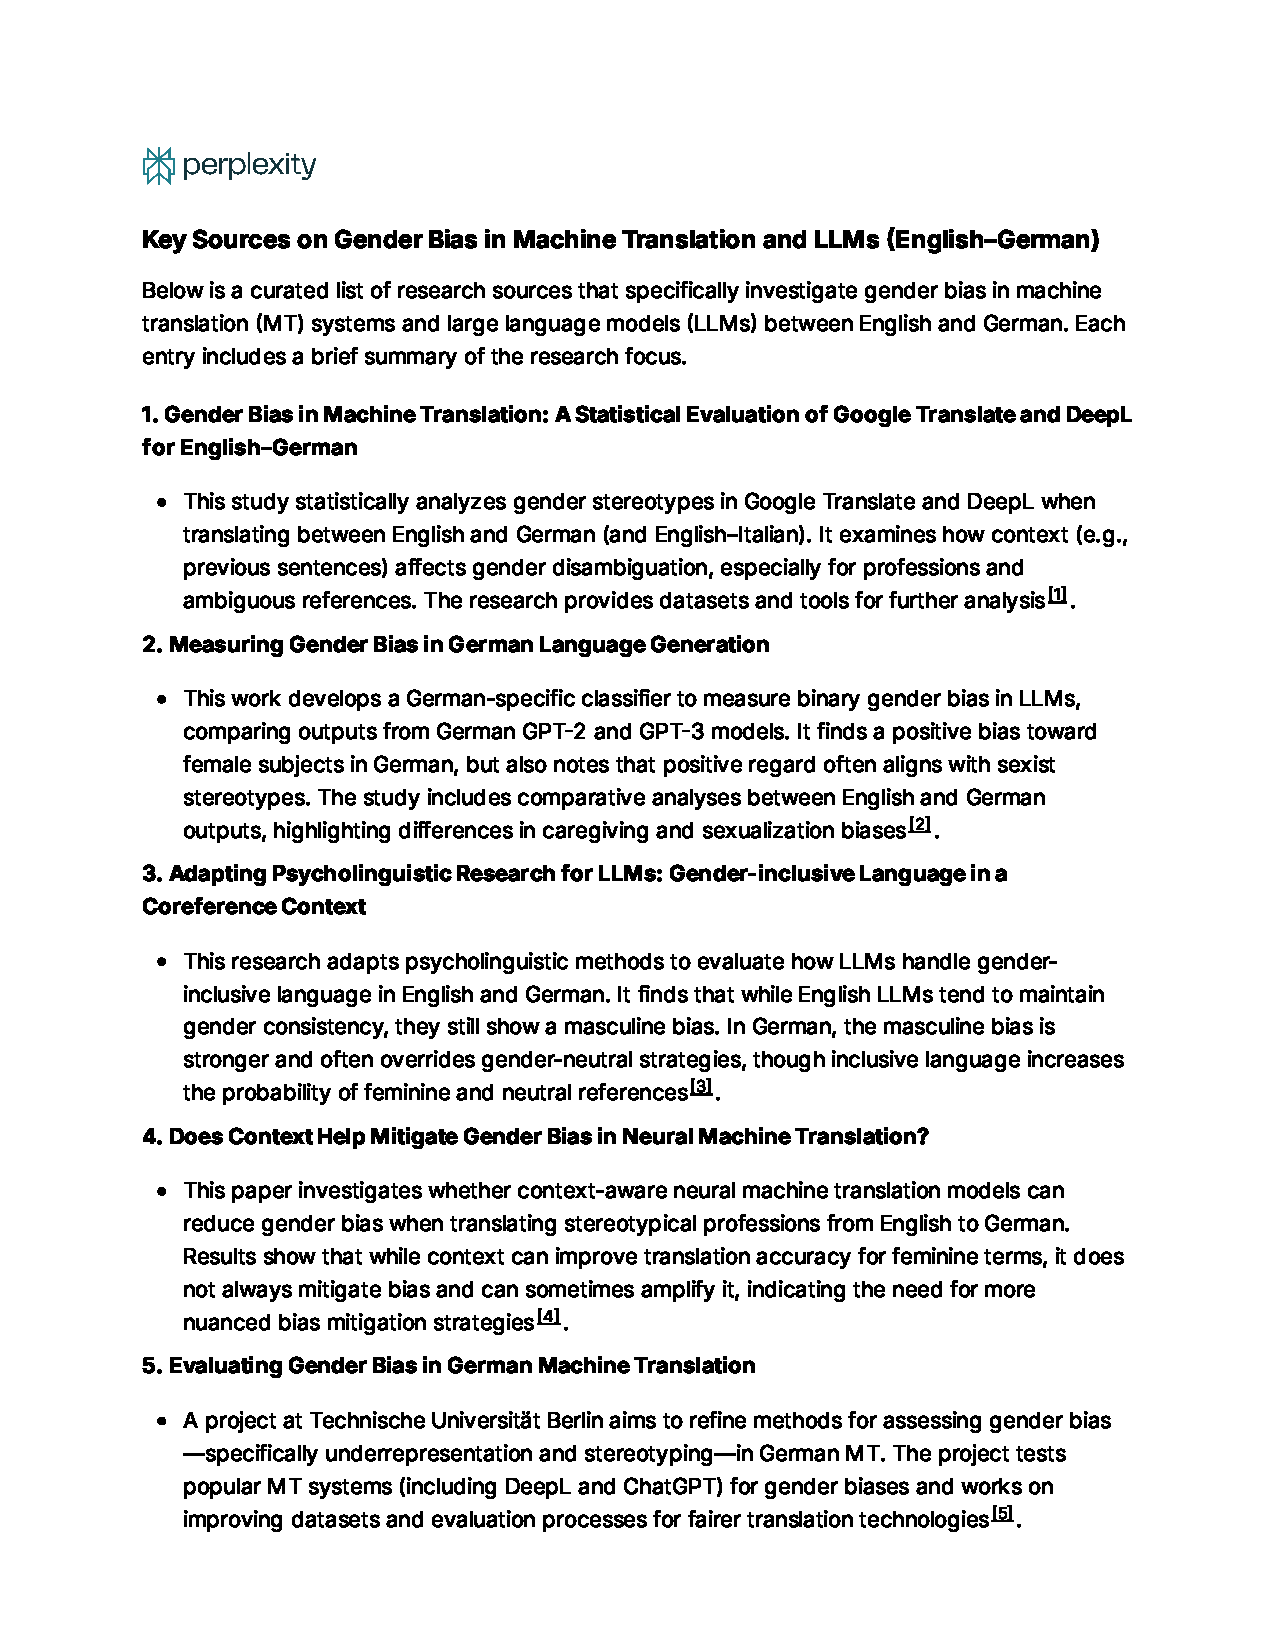
\includepdf[pages=-]{./Literatur/Key Sources on Gender Bias in Machine Translation 21-may-2025.pdf}

\subsection{Gemini for Synthetic Data Generation}\label{appendix:gemini_prompt}
Prompting Gemini to generate full sentences from the existing Building Bridges dataset \parencite{lardelliBuildingBridgesDataset2024}, which contained only nouns. I provided the lardelli\_singular.csv and lardelli\_plural.csv files as input. Manual sentence creation would have been too resource intensive. GPT and Deepseek were also tested, but they did not handle large amounts of data efficiently and only produced output in small batches. The final output was a singular output.csv, which I subsequently reviewed and corrected through additional manual rounds to fix errors.
\subsubsection{Prompt: } 

\begin{lstlisting}
Your Role: You are an expert linguist and data generation specialist. Your task is to create a high-quality structured dataset for ML by generating English sentences and their German translations based on two CSV files.

Goal: Process lardelli_singular.csv and lardelli_plural.csv to produce a final CSV with columns: english,german,label. Generate multiple variations per English sentence using different German translation rules.

Input Data:
lardelli_singular.csv: ID,German_MS,German_FS,Gender-Neutral,Gender-Inclusive,English,English_P
lardelli_plural.csv: ID,German_MP,German_FP,Gender-Neutral,Gender-Inclusive,English

Instructions:
1. Iterate through lardelli_singular.csv.
2. Generate 3-5 simple, correct English sentences for the singular noun (English) and plural noun (English_P). Create singular and plural versions.
Example: "The deputy is having a great day." / "The deputies are having a great day."
3. Generate German translations:
  - Singular: use current row.
    - Label 1: German_MS, German_FS
    - Label 0: Gender-Neutral, Gender-Inclusive
  - Plural: match ID in lardelli_plural.csv
    - Label 1: German_MP, German_FP
    - Label 0: Gender-Neutral, Gender-Inclusive
4. Quality rules:
  - Ensure grammatical correctness (articles, adjectives, verbs, case, number).
  - Skip missing values.
  - Generate all possible variants for balance.
  - English sentences should be varied.
  - Final CSV: english,german,label (use quotes if commas appear).

Example Output:
english,german,label
"The deputy is having a great day","Der Stellvertreter hat einen tollen Tag",1
"The deputy is having a great day","Die Stellvertreterin hat einen tollen Tag",1
"The deputy is having a great day","die Stellvertretung hat einen tollen Tag",0
"The deputy is having a great day","der*die Stellvertreter*in hat einen tollen Tag",0
"The deputies are having a great day","Die Stellvertreter haben einen tollen Tag",1
"The deputies are having a great day","Die Stellvertreterinnen haben einen tollen Tag",1
"The deputies are having a great day","Die Stellvertretung hat einen tollen Tag",0
"The deputies are having a great day","die Stellvertreter*innen haben einen tollen Tag",0

Begin generation now. If output is too large, produce in batches.

\end{lstlisting}

\subsubsection{Output: } 
\begin{lstlisting}
The data generation is complete, and the output has been saved to output_translations.csv. Overview of the process:

Loaded Data: The lardelli_singular.csv and lardelli_plural.csv files were loaded into DataFrames.

Sentence Generation: For each noun in lardelli_singular.csv, 3 singular and 3 plural English sentences were generated using simple, grammatically correct templates.

German Translation Generation: For each singular English sentence, corresponding German translations were generated using German_MS, German_FS, Gender-Neutral, and Gender-Inclusive columns from lardelli_singular.csv. For each plural English sentence, matching rows were found in lardelli_plural.csv using the ID, and German translations were generated using German_MP, German_FP, Gender-Neutral, and Gender-Inclusive columns. Translations were labeled as 1 (gendered) or 0 (neutral/inclusive). Rows with missing German translation values were skipped.

Output: All generated sentences and their translations were compiled into a single CSV file named output_translations.csv with columns english,german,label. Please find the generated CSV file below.

\end{lstlisting}

\subsection{Use of AI for Code Generation}\label{appendix:ai_code}
During the development of the practical part, I used ChatGPT and DeepSeek to assist in generating portions of the implementation for the demo, specifically in \texttt{app.py}, \texttt{utils.py}, and \texttt{translate.py}. The process involved multiple rounds of suggestions and refinements. All AI-generated code was reviewed, adapted, and integrated to ensure correctness and suitability for the project. AI assistance supported implementation but did not replace my own programming work or design decisions. Below is one example of AI-assisted code generation. Due to the iterative nature of the process, not all intermediate outputs can be shown. This example illustrates how AI was used to support the implementation.


\subsubsection{Prompt: } 

\begin{lstlisting}
look at my app.py: 
import streamlit as st
import torch
from transformers import BertTokenizer, BertForSequenceClassification
from utils import split_sentences, predict_bias_batch

device = torch.device("cuda" if torch.cuda.is_available() else "cpu")
MODEL_DIR = "./model_output" 
MAX_LENGTH = 128
BIAS_CONF_THRESHOLD = 0.9

@st.cache_resource(show_spinner=False)
def load_model_and_tokenizer():
    tokenizer = BertTokenizer.from_pretrained(MODEL_DIR)
    model = BertForSequenceClassification.from_pretrained(MODEL_DIR)
    model.to(device)
    model.eval()
    return tokenizer, model

tokenizer, model = load_model_and_tokenizer()

st.title("English to German Translation with Gender Bias Detection")
text = st.text_area("Enter English text here:")

if st.button("Translate"):
    if not text.strip():
        st.write("Please enter some text")
    else:
        st.write("### Results")
        sentences = split_sentences(text)
        results = predict_bias_batch(tokenizer, model, sentences, max_length=MAX_LENGTH, device=device, bias_threshold=BIAS_CONF_THRESHOLD)

        for sentence, translation, pred, conf in results:
            st.write(f"**english:** {sentence}")
            st.write(f"**german:** {translation}")
            if pred == 1 and conf >= BIAS_CONF_THRESHOLD:
                st.warning(f"Bias detected confidence: {conf:.2f}")
            else:
                st.success(f"No bias detected confidence: {conf:.2f}")
            st.markdown("---")

and utils.py:

import re
from translate import translate
import torch

def split_sentences(text):
    # split on . ! or ? followed by space(s)
    sentences = re.split(r'(?<=[.!?])\s+', text.strip())
    return [s for s in sentences if s]

def predict_bias_batch(tokenizer, model, sentences, max_length=128, device='cpu', bias_threshold=0.9):
    results = []
    for sentence in sentences:
        translation = translate(sentence)
        inputs = tokenizer(
            sentence,
            translation,
            return_tensors="pt",
            truncation=True,
            padding="max_length",
            max_length=max_length,
        )
        inputs = {k: v.to(device) for k, v in inputs.items()}
        with torch.no_grad():
            outputs = model(**inputs)
            probs = torch.softmax(outputs.logits, dim=1)
            pred = torch.argmax(probs, dim=1).item()
            confidence = probs[0][pred].item()
        results.append((sentence, translation, pred, confidence))
    return results

right now there is only one input field that utilises the translate script. i want another option that the user can choose to manually input translation, for example a tab selection. there are two input fields where the user inputs english and german and click a button "check bias". then the same standard bias detection script runs. you may add a new file or change existing ones
\end{lstlisting}

\subsubsection{Output:}
\begin{lstlisting}
To add the option for manual translation input, use Streamlit's `st.tabs` to create two modes:

1. **Translate Mode** (uses your `translate()` function).
2. **Manual Input Mode** (user provides both English and German text).

You only need to slightly update `app.py` and optionally refactor `predict_bias_batch` to handle one or more pairs directly. You do **not** need to change `utils.py` unless you want cleaner logic separation.

import streamlit as st
import torch
from transformers import BertTokenizer, BertForSequenceClassification
from utils import split_sentences, predict_bias_batch

device = torch.device("cuda" if torch.cuda.is_available() else "cpu")
MODEL_DIR = "./model_output"
MAX_LENGTH = 128
BIAS_CONF_THRESHOLD = 0.9

@st.cache_resource(show_spinner=False)
def load_model_and_tokenizer():
    tokenizer = BertTokenizer.from_pretrained(MODEL_DIR)
    model = BertForSequenceClassification.from_pretrained(MODEL_DIR)
    model.to(device)
    model.eval()
    return tokenizer, model

tokenizer, model = load_model_and_tokenizer()

st.title("Gender Bias Detection in English-German Translations")

tab1, tab2 = st.tabs(["Translate", "Manual Input"])

with tab1:
    text = st.text_area("Enter English text here:")
    if st.button("Translate and Check Bias"):
        if not text.strip():
            st.write("Please enter some text")
        else:
            st.write("### Results")
            sentences = split_sentences(text)
            results = predict_bias_batch(
                tokenizer,
                model,
                sentences,
                max_length=MAX_LENGTH,
                device=device,
                bias_threshold=BIAS_CONF_THRESHOLD,
                use_translation=True,
            )
            for sentence, translation, pred, conf in results:
                st.write(f"**english:** {sentence}")
                st.write(f"**german:** {translation}")
                if pred == 1 and conf >= BIAS_CONF_THRESHOLD:
                    st.warning(f"Bias detected confidence: {conf:.2f}")
                else:
                    st.success(f"No bias detected confidence: {conf:.2f}")
                st.markdown("---")

with tab2:
    manual_en = st.text_area("Enter English sentence:")
    manual_de = st.text_area("Enter German translation:")
    if st.button("Check Bias"):
        if not manual_en.strip() or not manual_de.strip():
            st.write("Please enter both English and German text")
        else:
            result = predict_bias_batch(
                tokenizer,
                model,
                [(manual_en, manual_de)],
                max_length=MAX_LENGTH,
                device=device,
                bias_threshold=BIAS_CONF_THRESHOLD,
                use_translation=False,
            )[0]
            sentence, translation, pred, conf = result
            st.write(f"**english:** {sentence}")
            st.write(f"**german:** {translation}")
            if pred == 1 and conf >= BIAS_CONF_THRESHOLD:
                st.warning(f"Bias detected confidence: {conf:.2f}")
            else:
                st.success(f"No bias detected confidence: {conf:.2f}")
\end{lstlisting}

\newpage
\thispagestyle{empty}
\chapter*{Declaration of Independent Work}

\noindent I hereby declare that I have written this thesis independently and have not used any sources or aids other than those indicated. The thesis has not been submitted in the same or similar form for any other examination. All verbatim or paraphrased passages, as well as any sections created, written, or edited with the help of AI-based tools, are clearly marked and cited. In the appendix of my thesis, I have listed all AI-based tools used, including product names and the prompts I employed, in an AI tools directory. I confirm that I have not used any AI-based tools whose use was explicitly prohibited by the examiner. I am aware that content generated by AI-based tools does not guarantee its quality. I take full responsibility for any machine-generated passages I have included and accept responsibility for any errors, distorted content, incorrect references, violations of data protection or copyright, or plagiarism resulting from the use of AI-generated content.


\vspace{2cm}

\noindent
Berlin, \today

\vspace{3cm}

\hspace*{7cm}%
\dotfill\\
\hspace*{8.5cm}%
\textit{(Signature)}
 			% Eidesstattliche Erklärung (nicht bei Seminararb.)

\end{document}